\chapter{系统架构与设计}

\section{硬件化改造需求分析}

在Rel4系统原有的实现中,异步系统调用的过程会经历特权级的切换和用户态中断的触发。具体过程大致如下:

异步系统调用的发起需要用户态的异步运行时以及异步系统调用库函数的支持。发起异步系统调用的协程是一个由异步运行时所调度的异步协程。在该协程提交异步系统调用后,库函数会将请求写入缓冲区,然后根据缓冲区中的原子变量判断内核中的处理协程是否正在执行。若内核中的处理协程已经空闲阻塞,则进行系统调用来唤醒内核中的处理协程。此时,CPU会陷入内核对该内核任务进行调度,并尝试寻找一个空闲的内核发送核间中断以执行该处理任务。综上,异步系统调用的发起引入了异步任务调度所需的必要开销以及两次特权级切换所带来的上下文保存恢复开销。

在处理协程完成异步系统调用处理后,内核会通过通知机制对调用方进程发送用户态中断,以唤醒用户态进程的中断处理函数。中断处理函数再调用接受回复的异步协程,对内核的回复进行分发。接受回复的异步协程会根据回复消息中的协程id,唤醒对应的因等待回复而阻塞的异步系统调用发起协程。此过程包含了用户态中断所带来的上下文保存恢复、中断处理函数中的协程唤醒,以及接受回复的异步协程进行的分发处理。

在整个异步系统调用的实现过程中,缓冲区的写入,读取,系统调用的实际处理是必要的。而此外,由于异步的引入,额外带来了(可能的)两次上下文切换开销,异步任务的调度开销,中断处理函数执行开销,以及回复分发的执行开销。

根据原Rel4异步系统调用的性能测试结果,在低并发场景下,异步系统调用的性能较低,且远高于同步。根据上文的过程分析可知,低并发场景下,内核中的处理协程有较大的概率处于空闲状态。这就导致CPU需要频繁的陷入内核以唤醒内核中的处理协程。同理,用户态中断的触发也会相较高并发场景更加频繁。由此可见,频繁的系统调用和用户态中断是导致低并发场景下异步系统调用性能较低的主要原因。
异步的引入旨在提高系统整体吞吐率,而低并发下高额的开销无法被较多的并发协程均摊。综上所述,Rel4中原有的异步系统调用需要性能优化,以减小异步功能的引入所带来的额外开销。

\section{异步系统调用的新架构}

为了减小上述过程所产生的不必要开销,我设计将Taic硬件调度器集成到Rel4操作系统中,用于代替异步运行时中原有依赖软件实现的调度逻辑。进而优化异步系统调用路径,改善整体的性能。

\subsection{异步运行时改造}

由xx结分析可以得知,Taic内部提供了多个硬件级的任务队列,具备跨特权级别的任务调度能力,即允许内核直接操作用户态调度上下文,而无需进行中断和陷入。基于这一特性,我首先对异步运行时进行了结构上的调整,将原本基于软件实现的协程阻塞与唤醒机制,替换为基于 Taic 队列的硬件实现。


\subsection{异步系统调用路径改造}

由于硬件调度器的引入,异步系统调用的提交不再需要通过原有的系统调用,也就无需陷入内核态进行相关处理。因此,我将异步调用的提交路径完全保留在用户态。利用taic队列的信号收发机制,直接在用户态将任务发送至内核控制流,大幅简化了路径、提升了执行效率。

同样的,内核处理完成后的回复消息也不再需要用户态中断进行间接唤醒。理想情况下,每个因等待内核回复而阻塞的异步发送协程均可被硬件直接唤醒。因此可以舍弃原有的分发协程与中断处理函数。但由于硬件唤醒的通道数量存在限制(xx小结中详述),我仍然保留了分发协程用于在高并发场景下,二次唤醒未成功申请到硬件通道的协程。

\subsection{系统调用完整流程}

根据上文的架构设计,改进后的异步系统调用流程如下:

\begin{enumerate}
  \item 在内核初始化时,会对异步运行时进行初始化。该过程中会调用taic相关接口分配资源,申请一个内核专用的队列。
  \item 在创建用户态进程时,异步运行时会申请Taic队列,创建缓冲区,并完成的异步系统调用的注册。此时内核会创建一个单独的处理该用户态进程异步系统调用的协程,并将该协程加入阻塞队列。
  \item 当用户态进程需要发起异步系统调用时,会创建一个异步协程。该协程会构造请求消息并将消息写入缓冲区。随后根据内核中的执行情况,调用硬件能力唤醒内核协程。一切准备就绪会,该协程会阻塞自身,等待回复
  \item 内核执行处理异步系统调用的协程。该协程会从缓冲区中读取消息,进行处理并将结果写回缓冲区。随后,根据协程的id以及分发协程的执行情况,唤醒对应的协程。
  \item 用户态阻塞等待回复的协程因唤醒而被调度执行。该协程会从缓冲区收到回复,至此一次完整的异步系统调用完成。
\end{enumerate}

\section{异步运行时的硬件适配}

\subsection{系统架构设计}

为了将Taic引入到异步运行时中,我设计采用分层架构,如图 X 所示,系统结构从上至下依次为:内核/用户态程序、异步运行时、Taic接口层、Taic驱动层以及最底层的Taic硬件。

内核态与用户态中的异步程序位于最上层,可直接通过异步语义发起异步系统调用。异步协程的阻塞、唤醒与调度由下层的异步运行时负责管理,从而实现了异步过程的自动化控制。

为了更好的在异步运行时中调用硬件调度器的能力,我设计增加了一层Taic接口层作为运行时与底层驱动之间的抽象桥梁。该层提供统一接口和地址映射功能,在Taic原有驱动的基础上进行了进一步的封装,实现了支持跨越特权级的任务控制操作。

\subsection{相关接口调整}

在原有的初始化过程中,加入硬件能力的初始化。
替换异步运行时的就绪队列为一个硬件结构抽象出的队列对象。

\section{硬件资源分配与映射策略}

\subsection{中断向量映射策略}

在3.2章节中所叙述的优化框架中,协程需要被一一对应的唤醒。由2.2.3中所阐述的Taic模型可知,协程的唤醒需要通过队列中提前分配的“中断向量”。Taic硬件调度器仅提供固定数量的中断向量(共32个),因此,如何在有限的中断资源下高效地映射和调度大量用户态协程,成为本设计中的核心问题之一。为尽可能高效的利用已有的硬件资源并提高低并发下的异步性能。本设计采用动态映射策略分配中断向量。

该设计在异步运行时中保留一个0号协程(dispatcher协程)。该协程常驻于异步运行时中,用于在硬件资源不足时间接唤醒协程,以实现硬件资源的复用。

在客户端执行异步系统调用请求的过程中,请求协程首先尝试向申请空闲向量,用于在内核完成操作后反向唤醒自身。

\begin{itemize}
  \item 若当前中断向量表尚未满载,即存在可用中断向量,则会成功分配到一个向量号。协程会将该中断向量写入调用传递的消息中,连同其他上下文信息发送给内核。当内核处理完毕后,即可通过该中断向量向对原始协程的直接唤醒,无需额外中间调度,极大提升响应效率。

  \item 若中断向量表已满,即所有中断向量已被活跃协程占用,当前协程无法获得中断资源。此时,协程会将消息结构中的中断向量字段显式置0,表明该请求不绑定硬件中断唤醒。内核在处理完该请求后,会将该请求的回复消息id加入缓冲区中的控制队列(3.5章节中有叙述),并尝试唤醒dispatcher协程。dispatcher协程在被唤醒后,解析消息中的相关字段并唤醒对应的用户协程,完成该异步系统调用的回复流程。
\end{itemize}

中断向量的管理由硬件接口层负责。在系统初始化阶段,硬件接口层在内存中构建并初始化中断向量表结构。该向量表采用位图方式存储中断向量的分配状态,其中0号中断向量被保留用于唤醒0号协程。同时,接口层向上层提供向量申请与释放接口,从而实现硬件资源的动态分配。

该映射机制有效地实现了对硬件接口的封装与抽象。整个过程由异步运行时与硬件接口层协同完成,上层应用代码无需感知底层实现细节。

\section{异步通信缓冲区结构优化}\label{sec:buffer}

原有的缓冲区采用环形队列实现消息的存储与管理。为了更好的适配新的处理流程并提高异步性能,我对缓冲区的结构设计进行了重新设计与优化。

由于在硬件资源充足的情况下取消了dispatcher协程的分发过程,原阻塞协程直接由内核唤醒。这一变更虽然减少了调度开销,但也带来了新的挑战:由于消息处理的顺序不再严格遵循写入顺序,原有的环形队列已不再适应这种处理模式。因此,我将缓冲区的结构由环形队列改为基于“消息槽”的形式,并设计了一套槽位分配机制,尽可能的降低写入和读取所造成的开销。

新的缓冲区由数据区、索引队列和状态变量三部分组成。

\begin{figure}[htbp]
  \centering
  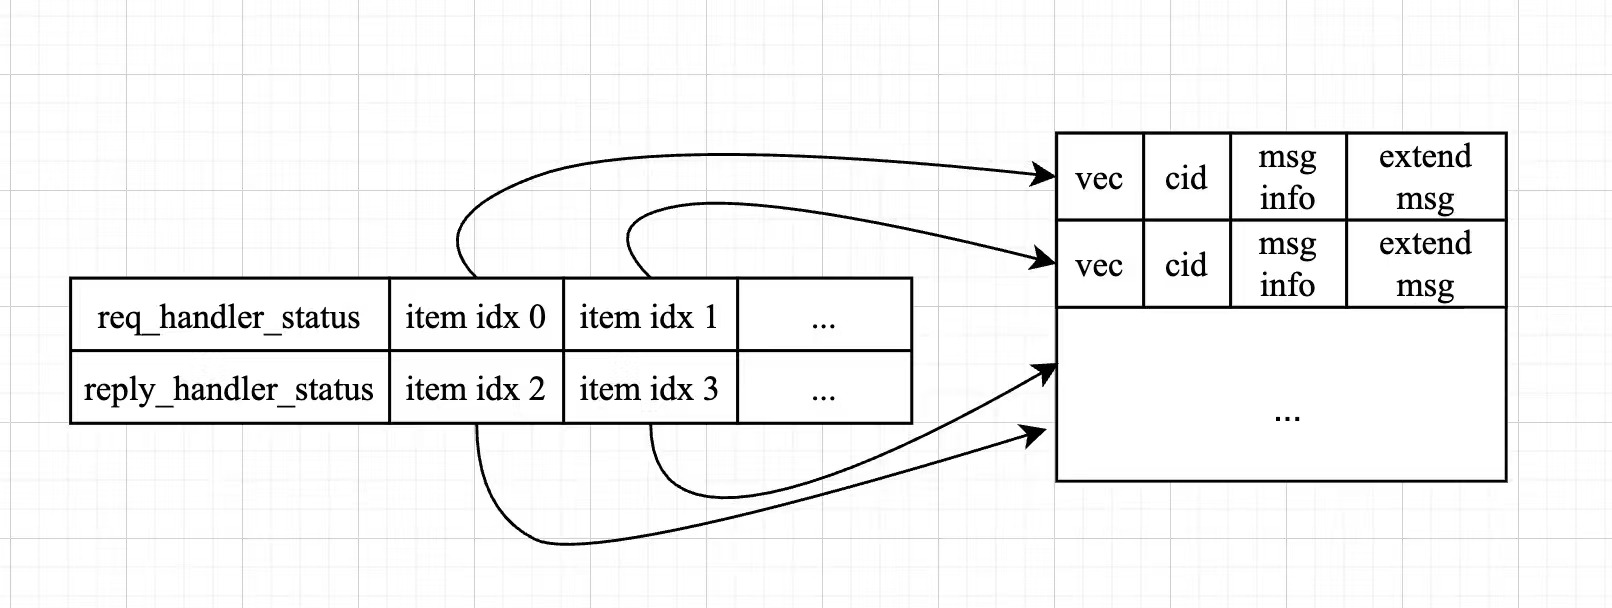
\includegraphics[width=0.8\textwidth]{images/buffer_structure.jpg}
  \caption{缓冲区结构示意图}\label{缓冲区结构示意图}
\end{figure}

数据区是一个预分配的内存块,用于存储异步系统调用过程中传递的消息。整个区域被划分为多个“消息槽”,每个槽用于存储一条完整的消息内容。

索引队列包括数据区的控制信息。索引队列中存储着需要内核协程处理的请求消息id和需要分发协程分发的消息的id。协程可以从队列中依次取出需要处理的消息id,然后根据该 ID 从数据区中读取相应的消息内容,进行处理或分发。

状态变量由两个原子标志组成,分别表示内核中的处理协程和用户态的回复分发协程是否阻塞。

当协程发起异步系统调用时,首先会向缓冲区申请一个槽位id,然后将消息写入数据区对应的位置并将该消息的id入队。内核处理协程在执行过程中,会从队列中取出待处理的消息id,读取对应槽中的数据进行处理,并将处理结果写回同一槽位。

当硬件资源充足时,回复消息不需要经过分发协程分发,因此不需要将回复的消息id入队。若并发数超过31,部分协程不能直接通过硬件唤醒,则需要将回复的消息id写入队列。并尝试唤醒分发协程。分发协程同样会依次取出队列中的消息id,然后根据消息的id读取数据区的消息,进而再唤醒对应的协程。

\section{异步事件注册机制的应用}

由3.5节叙述可知,协程的中断向量采用了动态分配的策略,中断向量的注册是在运行时进行的。而中断向量的注册机制会对异步系统的实时性造成影响。如第2.2.x节所述,Taic提供了两种中断注册方式:“一次性注册”与“持续注册”。

默认的注册机制采用“一次性注册”策略:每当协程因中断事件被唤然而,在高并发或高频唤醒中,频繁注册与注销事件会带来非忽略的开销,影响整体调度性能。

为优化上述问题,Taic提供了一种基于标志位控制的“持续注册”机制。在该模式下,开发者可通过设置注册参数中的特定标志位,实现中断向量的保留与复用,避免不必要的重复注册。此机制在高并发或重复事件场景下具有显著优势,能有效减少调度延迟与资源竞争。但在中断频度较低或并发度不高的系统中,可能会限制灵活性。

基于上述两种机制,本设计均进行了完整实现,并构建了相应的测试用例用于功能验证与性能评估。具体的实验配置、对比分析与测试结果将在第5.3节中详述。



\section{本章小结}

本章围绕Rel4异步系统调用的性能瓶颈,分析了其在低并发场景下性能下降的主要原因,指出频繁的特权级切换与用户态中断是系统开销的重要来源。针对这一问题,设计并引入了Taic硬件调度器,替代原有软件调度逻辑,从而重构了异步系统调用路径。本章详细描述了异步运行时与系统调用流程的改造方法,提出了支持硬件调度的异步运行时架构。随后,介绍了中断向量的动态分配策略及其在硬件资源受限情况下的调度优化机制,并对缓冲区结构进行了适配与重构,以支持新的唤醒模式。最后,分析了异步事件注册机制的两种实现方式,并为后续实验验证做了准备。